\documentclass[journal,12pt,onecolumn]{IEEEtran}
\usepackage{cite}
 \usepackage{caption}
\usepackage{graphicx}
\usepackage{amsmath,amssymb,amsfonts,amsthm}
\usepackage{algorithmic}
\usepackage{graphicx}
\usepackage{textcomp}
\usepackage{xcolor}
\usepackage{txfonts}
\usepackage{listings}
\usepackage{enumitem}
\usepackage{mathtools}
\usepackage{gensymb}
\usepackage{comment}
\usepackage[breaklinks=true]{hyperref}
\usepackage{tkz-euclide} 
\usepackage{listings}
\usepackage{gvv}
%\def\inputGnumericTable{}                                 
\usepackage[latin1]{inputenc} 
\usetikzlibrary{arrows.meta, positioning}
\usepackage{xparse}
\usepackage{color}                                            
\usepackage{array}                                            
\usepackage{longtable}                                       
\usepackage{calc}                                             
\usepackage{multirow}
\usepackage{multicol}
\usepackage{hhline}                                           
\usepackage{ifthen}                                           
\usepackage{lscape}
\usepackage{tabularx}
\usepackage{array}
\usepackage{float}

\usepackage{float}
%\newcommand{\define}{\stackrel{\triangle}{=}}
\theoremstyle{remark}
\usepackage{circuitikz}
\captionsetup{justification=centering}
\usepackage{tikz}

\title{Matrices in Geometry 2.4.32}
\author{EE25BTECH11035 - Kushal B N}
\begin{document}
\vspace{3cm}
\maketitle
{\let\newpage\relax\maketitle}
\textbf{Question: }
The points $\vec{A}\brak{-1,-2}$, $\vec{B}\brak{4,3}$, $\vec{C}\brak{2,5}$ and $\vec{D}\brak{-3,0}$ in that order form a rectangle.

\textbf{Given: } \\
$\vec{A}\myvec{-1\\-2}$, $\vec{B}\myvec{4\\3}$, $\vec{C}\myvec{2\\5}$ and $\vec{D}\myvec{-3\\0}$

\textbf{Solution: }\\
\begin{equation}
\vec{B} - \vec{A} = \myvec{5\\5}
\end{equation}

\begin{equation}
\vec{C} - \vec{B} = \myvec{-2\\2}
\end{equation}

\begin{equation}
\vec{D} - \vec{C} = \myvec{-5\\-5}
\end{equation}

\begin{equation}
\vec{A} - \vec{D} = \myvec{2\\-2}
\end{equation}

Checking opposite sides,\\
\begin{equation}
\brak{\vec{B} - \vec{A}} = - \brak{\vec{D} - \vec{C}}
\end{equation}

Now, as each pair of opposite sides are parallel and equal in length, this means that the given points make up a parallelogram.\\
Checking for right angle, we need to check for inner product of the adjacent sides of the parallelogram.\\

\begin{equation}
\brak{\vec{B}-\vec{A}}^{\top}\brak{\vec{C}-\vec{B}} = \myvec{5 & 5}\myvec{-2\\2} = 0
\end{equation}

This implies that the angle at B is a right angle. A parallelogram with a right angle is a rectangle.
Checking for square:\\
The given quadrilateral will be a square if its diagonals are orthogonal.

\begin{equation}
    \brak{\vec{C}-\vec{A}}^{\top}\brak{\vec{D}-\vec{B}} = \myvec{3&7}\myvec{-7\\-3} = -42
\end{equation}

From $\brak{7}$, we can see that $\brak{\vec{C}-\vec{A}}^{\top}\brak{\vec{D}-\vec{B}} \neq 0$, that is the diagonals are not orthogonal and hence the given quadrilateral cannot be a square.\\

$\therefore$ The quadrilateral $\vec{ABCD}$ is a rectangle.

\begin{figure}[H]
    \centering
    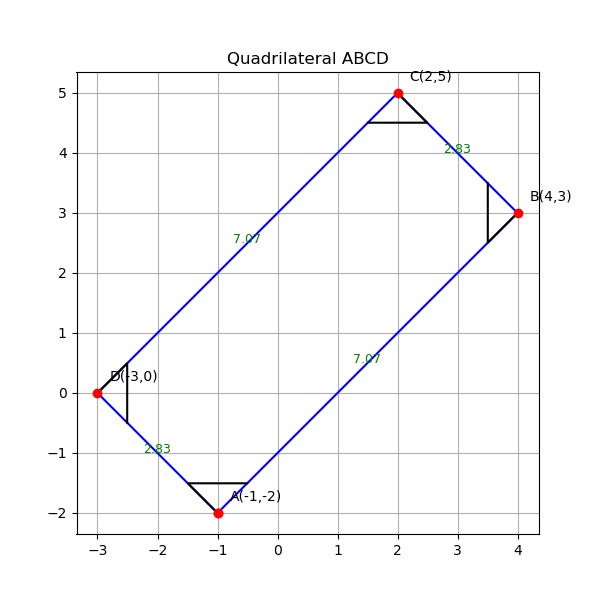
\includegraphics[width=1\columnwidth]{figs/1.png}
    \caption{Plot for 2.4.32}
    \label{fig:placeholder}
\end{figure}


\end{document}
